%!TEX program = xelatex
%# -*- coding: utf-8 -*-
%!TEX encoding = UTF-8 Unicode

\documentclass[12pt,oneside,a4paper]{article}\usepackage[]{graphicx}\usepackage[]{xcolor}
%% maxwidth is the original width if it is less than linewidth
%% otherwise use linewidth (to make sure the graphics do not exceed the margin)
\makeatletter
\def\maxwidth{ %
  \ifdim\Gin@nat@width>\linewidth
    \linewidth
  \else
    \Gin@nat@width
  \fi
}
\makeatother

\definecolor{fgcolor}{rgb}{0, 0, 0}
\newcommand{\hlnum}[1]{\textcolor[rgb]{0,0,0}{#1}}%
\newcommand{\hlstr}[1]{\textcolor[rgb]{0,0,1}{#1}}%
\newcommand{\hlcom}[1]{\textcolor[rgb]{0.443,0.478,0.702}{#1}}%
\newcommand{\hlopt}[1]{\textcolor[rgb]{0,0,0}{#1}}%
\newcommand{\hlstd}[1]{\textcolor[rgb]{0,0,0}{#1}}%
\newcommand{\hlkwa}[1]{\textcolor[rgb]{0.498,0,0.333}{\textbf{#1}}}%
\newcommand{\hlkwb}[1]{\textcolor[rgb]{0.498,0,0.333}{\textbf{#1}}}%
\newcommand{\hlkwc}[1]{\textcolor[rgb]{0.498,0,0.333}{\textbf{#1}}}%
\newcommand{\hlkwd}[1]{\textcolor[rgb]{0,0,0}{#1}}%

\usepackage{framed}
\makeatletter
\newenvironment{kframe}{%
 \def\at@end@of@kframe{}%
 \ifinner\ifhmode%
  \def\at@end@of@kframe{\end{minipage}}%
  \begin{minipage}{\columnwidth}%
 \fi\fi%
 \def\FrameCommand##1{\hskip\@totalleftmargin \hskip-\fboxsep
 \colorbox{shadecolor}{##1}\hskip-\fboxsep
     % There is no \\@totalrightmargin, so:
     \hskip-\linewidth \hskip-\@totalleftmargin \hskip\columnwidth}%
 \MakeFramed {\advance\hsize-\width
   \@totalleftmargin\z@ \linewidth\hsize
   \@setminipage}}%
 {\par\unskip\endMakeFramed%
 \at@end@of@kframe}
\makeatother

\definecolor{shadecolor}{rgb}{.97, .97, .97}
\definecolor{messagecolor}{rgb}{0, 0, 0}
\definecolor{warningcolor}{rgb}{1, 0, 1}
\definecolor{errorcolor}{rgb}{1, 0, 0}
\newenvironment{knitrout}{}{} % an empty environment to be redefined in TeX

\usepackage{alltt}
\usepackage{geometry}
\geometry{verbose,tmargin=2cm,bmargin=2cm,lmargin=2cm,rmargin=2cm}
\usepackage[pdfusetitle,
 bookmarks=true,bookmarksnumbered=true,bookmarksopen=true,bookmarksopenlevel=2,
 breaklinks=false,pdfborder={0 0 1},backref=false,colorlinks=false]
 {hyperref}
\hypersetup{pdfstartview={XYZ null null 1}}
\usepackage{url}
\setcounter{secnumdepth}{2}
\setcounter{tocdepth}{2}
\usepackage{microtype}

\usepackage{amsmath, amsthm, amssymb, amsfonts}
\usepackage[retainorgcmds]{IEEEtrantools}

\usepackage{algorithm}
\usepackage{algorithmic}
\renewcommand{\algorithmicrequire}{\textbf{Input:}} 
\renewcommand{\algorithmicensure}{\textbf{Output:}} 
 
\usepackage[sc]{mathpazo}
\linespread{1.1}
\usepackage[T1]{fontenc}

\usepackage{graphics}
\usepackage{graphicx}
\usepackage[figure]{hypcap}
\usepackage[hypcap]{caption}
\usepackage{tikz}
%\usepackage{grffile} 
%\usepackage{float} 
\usepackage{pdfpages}

\usepackage{multirow}
\usepackage{booktabs}
\usepackage{threeparttable}

%\usepackage[square,numbers,super,comma,sort]{natbib}
%\usepackage[backend=biber, style=nature, sorting=none, isbn=false, url=false, doi=false]{biblatex}
%\addbibresource{ref.bib}
%\usepackage[]{authblk}

\usepackage{verbatim}

\newcommand{\problem}[1]
{
    \clearpage
    \section*{Problem {#1}}
}

\newcommand{\subproblem}[1]
{
    \subsection*{Problem {#1}}
}


\newcommand{\solution}
{
    \vspace{15pt}
    \noindent\ignorespaces\textbf{\large Solution}\par
}

\usepackage{fancyhdr}
\usepackage{extramarks}
\lhead{\hmwkAuthorName}
\chead{\hmwkTitle}
\rhead{\firstxmark}
\cfoot{\thepage}

\newcommand{\hmwkTitle}{STAT 8051 HW 8}
\newcommand{\hmwkAuthorName}{Jingxiang Li}

\setlength\headheight{15pt}
\setlength\parindent{0pt}
\setlength{\parskip}{0.5em}

\newcommand{\m}[1]{\texttt{{#1}}}
\newcommand{\E}[0]{\mathrm{E}}
\newcommand{\Var}[0]{\mathrm{Var}}
\newcommand{\Cov}[0]{\mathrm{Cov}}



\pagestyle{fancy}

\title{\hmwkTitle}
\author{\hmwkAuthorName}
\date{\today}
\IfFileExists{upquote.sty}{\usepackage{upquote}}{}
\begin{document}

\maketitle



\problem{1}
The dataset discoveries lists the numbers of ``great'' inventions and scientific discoveries in each year from 1860 to 1959. Has the discovery rate remained constant over time?

\solution
To test whether the discovery rate remained constant over time, we decide to use Pearson's chi-squared test to evaluate how likely it is that any observed difference arose by chance. However, the number of ``great'' inventions for each year is very small, thus we can't directly apply Pearson's chi-squared test to the original dataset, we have to combine some observations and let each ``combined observation'' have higher frequency value.  

\begin{table}[ht!]
\centering
\caption{Combined Data}
\begin{tabular}{cc}
\toprule
 \multicolumn{1}{c}{ Observation } & \multicolumn{1}{c}{ Expectation } \\
\midrule
 $18$ & $24.8$ \\
 $16$ & $21.7$ \\
 $17$ & $15.5$ \\
 $16$ & $15.5$ \\
 $25$ & $9.3$ \\
 $21$ & $12.4$ \\
 $21$ & $15.5$ \\
 $16$ & $15.5$ \\
 $17$ & $18.6$ \\
 $19$ & $15.5$ \\
 $17$ & $9.3$ \\
 $17$ & $18.6$ \\
 $17$ & $12.4$ \\
 $20$ & $15.5$ \\
 $16$ & $24.8$ \\
 $18$ & $27.9$ \\
 $16$ & $21.7$ \\
 $3$ & $15.5$ \\
\bottomrule
\end{tabular}
\label{tab:combinedData}
\end{table}

Table \ref{tab:combinedData} is the combined data. Then, we are going to apply Pearson's chi-squared test to the combined dataset and see whether the discovery rate remained constant over time.
\clearpage
\begin{knitrout}
\definecolor{shadecolor}{rgb}{1, 1, 1}\color{fgcolor}\begin{kframe}
\begin{alltt}
\hlkwd{require}\hlstd{(faraway)}
\hlkwd{require}\hlstd{(MASS)}

\hlstd{data} \hlkwb{<-} \hlstd{discoveries}
\hlstd{E_x} \hlkwb{<-} \hlkwd{sum}\hlstd{(data)} \hlopt{/} \hlkwd{length}\hlstd{(data)} \hlcom{## Expectation under constant discovery rate}

\hlcom{## build up the combined data}
\hlstd{k} \hlkwb{=} \hlnum{1}
\hlstd{x} \hlkwb{=} \hlkwd{vector}\hlstd{(}\hlkwc{mode} \hlstd{=} \hlstr{"numeric"}\hlstd{,} \hlkwc{length} \hlstd{=} \hlkwd{length}\hlstd{(data))}
\hlstd{y} \hlkwb{=} \hlstd{x}
\hlkwa{for} \hlstd{(i} \hlkwa{in} \hlnum{1}\hlopt{:}\hlkwd{length}\hlstd{(data))}
\hlstd{\{}
    \hlstd{x[k]} \hlkwb{<-} \hlstd{x[k]} \hlopt{+} \hlstd{data[i]}
    \hlstd{y[k]} \hlkwb{<-} \hlstd{y[k]} \hlopt{+} \hlnum{1}

    \hlkwa{if} \hlstd{(x[k]} \hlopt{>} \hlnum{15}\hlstd{)}
    \hlstd{\{}
        \hlstd{k} \hlkwb{<-} \hlstd{k} \hlopt{+} \hlnum{1}
    \hlstd{\}}
\hlstd{\}}

\hlstd{n} \hlkwb{<-} \hlkwd{sum}\hlstd{(x} \hlopt{>} \hlnum{0}\hlstd{)}
\hlstd{x} \hlkwb{<-} \hlstd{x[}\hlnum{1} \hlopt{:} \hlstd{n]} \hlcom{## Observation for combined data}
\hlstd{y} \hlkwb{<-} \hlstd{y[}\hlnum{1} \hlopt{:} \hlstd{n]}
\hlstd{EE_x} \hlkwb{<-} \hlstd{y} \hlopt{*} \hlstd{E_x} \hlcom{## Expectation for combined data}

\hlcom{## Apply Pearson's chi-squared test to the combined data}
\hlkwd{chisq.test}\hlstd{(}\hlkwc{x} \hlstd{= x,} \hlkwc{p} \hlstd{= EE_x,} \hlkwc{rescale.p} \hlstd{=} \hlnum{TRUE}\hlstd{)}
\end{alltt}
\begin{verbatim}
## 
## 	Chi-squared test for given probabilities
## 
## data:  x
## X-squared = 66.6267, df = 17, p-value = 8.146e-08
\end{verbatim}
\end{kframe}
\end{knitrout}

here we see the resulting p-value is $8.146\textrm{e}-08$, which suggests that the discovery rate did not remain constant over time.

\problem{2}
The salmonella data was collected in a salmonella reverse mutagenicity assay. The predictor is the dose level of quinoline and the response is the numbers of revertant colonies of TA98 salmonella observed on each of three replicate plates. Show that a Poisson GLM is inadequate and that some overdispersion must be allowed for. Do not forget to check out other reasons for a high deviance.

\solution
\begin{knitrout}
\definecolor{shadecolor}{rgb}{1, 1, 1}\color{fgcolor}\begin{kframe}
\begin{alltt}
\hlstd{data} \hlkwb{<-} \hlstd{salmonella}
\hlstd{m1} \hlkwb{<-} \hlkwd{glm}\hlstd{(colonies} \hlopt{~} \hlstd{dose,} \hlkwc{family} \hlstd{= poisson,} \hlkwc{data} \hlstd{= data)}
\hlkwd{summary}\hlstd{(m1)}
\end{alltt}
\begin{verbatim}
## 
## Call:
## glm(formula = colonies ~ dose, family = poisson, data = data)
## 
## Deviance Residuals: 
##     Min       1Q   Median       3Q      Max  
## -2.6482  -1.8225  -0.2993   1.2917   5.1861  
## 
## Coefficients:
##              Estimate Std. Error z value Pr(>|z|)    
## (Intercept) 3.3219950  0.0540292  61.485   <2e-16 ***
## dose        0.0001901  0.0001172   1.622    0.105    
## ---
## Signif. codes:  0 '***' 0.001 '**' 0.01 '*' 0.05 '.' 0.1 ' ' 1
## 
## (Dispersion parameter for poisson family taken to be 1)
## 
##     Null deviance: 78.358  on 17  degrees of freedom
## Residual deviance: 75.806  on 16  degrees of freedom
## AIC: 172.34
## 
## Number of Fisher Scoring iterations: 4
\end{verbatim}
\begin{alltt}
\hlkwd{par}\hlstd{(}\hlkwc{mfrow} \hlstd{=} \hlkwd{c}\hlstd{(}\hlnum{1}\hlstd{,} \hlnum{2}\hlstd{))}
\hlkwd{halfnorm}\hlstd{(}\hlkwd{residuals}\hlstd{(m1),} \hlkwc{main} \hlstd{=} \hlstr{"Half-normal Plot"}\hlstd{)}
\hlkwd{plot}\hlstd{(}\hlkwd{log}\hlstd{(}\hlkwd{fitted}\hlstd{(m1)),} \hlkwd{log}\hlstd{((data}\hlopt{$}\hlstd{colonies} \hlopt{-} \hlkwd{fitted}\hlstd{(m1))}\hlopt{^}\hlnum{2}\hlstd{),}
     \hlkwc{xlab} \hlstd{=} \hlkwd{expression}\hlstd{(}\hlkwd{hat}\hlstd{(mu)),} \hlkwc{ylab} \hlstd{=} \hlkwd{expression}\hlstd{((y} \hlopt{-} \hlkwd{hat}\hlstd{(mu))}\hlopt{^}\hlnum{2}\hlstd{),}
     \hlkwc{main} \hlstd{=} \hlstr{"Variance VS. Mean"}\hlstd{)}
\hlkwd{abline}\hlstd{(}\hlnum{0}\hlstd{,} \hlnum{1}\hlstd{)}
\end{alltt}
\end{kframe}

{\centering 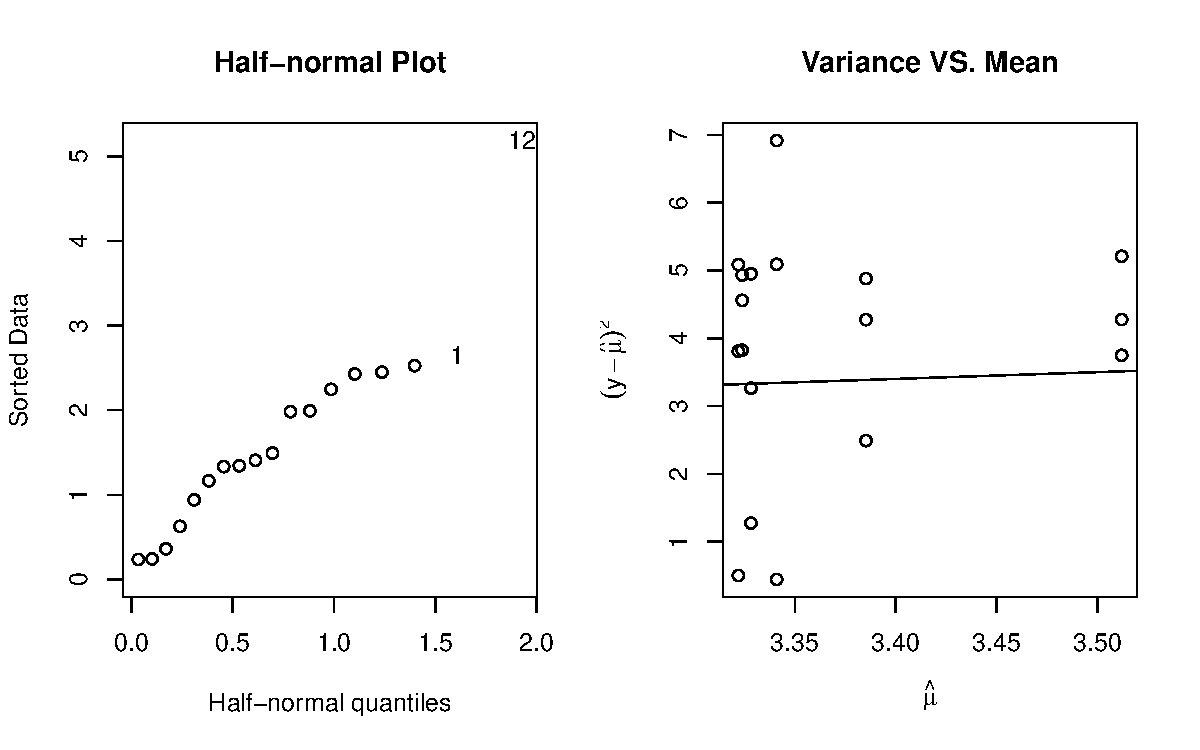
\includegraphics[width=1\linewidth]{figure/p2_1-1} 

}



\end{knitrout}

Here we see the resulting residual deviance is 75.81 with 16 degrees of freedom which indicates an ill-fitting model if the Poisson is the correct model for the response. First we check outliers for the model by Half-normal plot. In the plot above we see that case 12 is vary likely to be an outlier, so we remove it and rebuild the Poisson regression.

\begin{knitrout}
\definecolor{shadecolor}{rgb}{1, 1, 1}\color{fgcolor}\begin{kframe}
\begin{alltt}
\hlstd{data1} \hlkwb{<-} \hlstd{data[}\hlopt{-}\hlnum{12}\hlstd{, ]}
\hlstd{m1} \hlkwb{<-} \hlkwd{update}\hlstd{(m1,} \hlkwc{data} \hlstd{= data1)}
\hlkwd{summary}\hlstd{(m1)}
\end{alltt}
\begin{verbatim}
## 
## Call:
## glm(formula = colonies ~ dose, family = poisson, data = data1)
## 
## Deviance Residuals: 
##      Min        1Q    Median        3Q       Max  
## -2.49190  -1.54866   0.08807   1.40904   2.70520  
## 
## Coefficients:
##              Estimate Std. Error z value Pr(>|z|)    
## (Intercept) 3.2317358  0.0582053  55.523   <2e-16 ***
## dose        0.0002739  0.0001197   2.289   0.0221 *  
## ---
## Signif. codes:  0 '***' 0.001 '**' 0.01 '*' 0.05 '.' 0.1 ' ' 1
## 
## (Dispersion parameter for poisson family taken to be 1)
## 
##     Null deviance: 51.379  on 16  degrees of freedom
## Residual deviance: 46.347  on 15  degrees of freedom
## AIC: 136.95
## 
## Number of Fisher Scoring iterations: 4
\end{verbatim}
\begin{alltt}
\hlkwd{par}\hlstd{(}\hlkwc{mfrow} \hlstd{=} \hlkwd{c}\hlstd{(}\hlnum{1}\hlstd{,} \hlnum{2}\hlstd{))}
\hlkwd{halfnorm}\hlstd{(}\hlkwd{residuals}\hlstd{(m1),} \hlkwc{main} \hlstd{=} \hlstr{"Half-normal Plot"}\hlstd{)}
\hlkwd{plot}\hlstd{(}\hlkwd{log}\hlstd{(}\hlkwd{fitted}\hlstd{(m1)),} \hlkwd{log}\hlstd{((data1}\hlopt{$}\hlstd{colonies} \hlopt{-} \hlkwd{fitted}\hlstd{(m1))}\hlopt{^}\hlnum{2}\hlstd{),}
     \hlkwc{xlab} \hlstd{=} \hlkwd{expression}\hlstd{(}\hlkwd{hat}\hlstd{(mu)),} \hlkwc{ylab} \hlstd{=} \hlkwd{expression}\hlstd{((y} \hlopt{-} \hlkwd{hat}\hlstd{(mu))}\hlopt{^}\hlnum{2}\hlstd{),}
     \hlkwc{main} \hlstd{=} \hlstr{"Variance VS. Mean"}\hlstd{)}
\hlkwd{abline}\hlstd{(}\hlnum{0}\hlstd{,} \hlnum{1}\hlstd{)}
\end{alltt}
\end{kframe}

{\centering 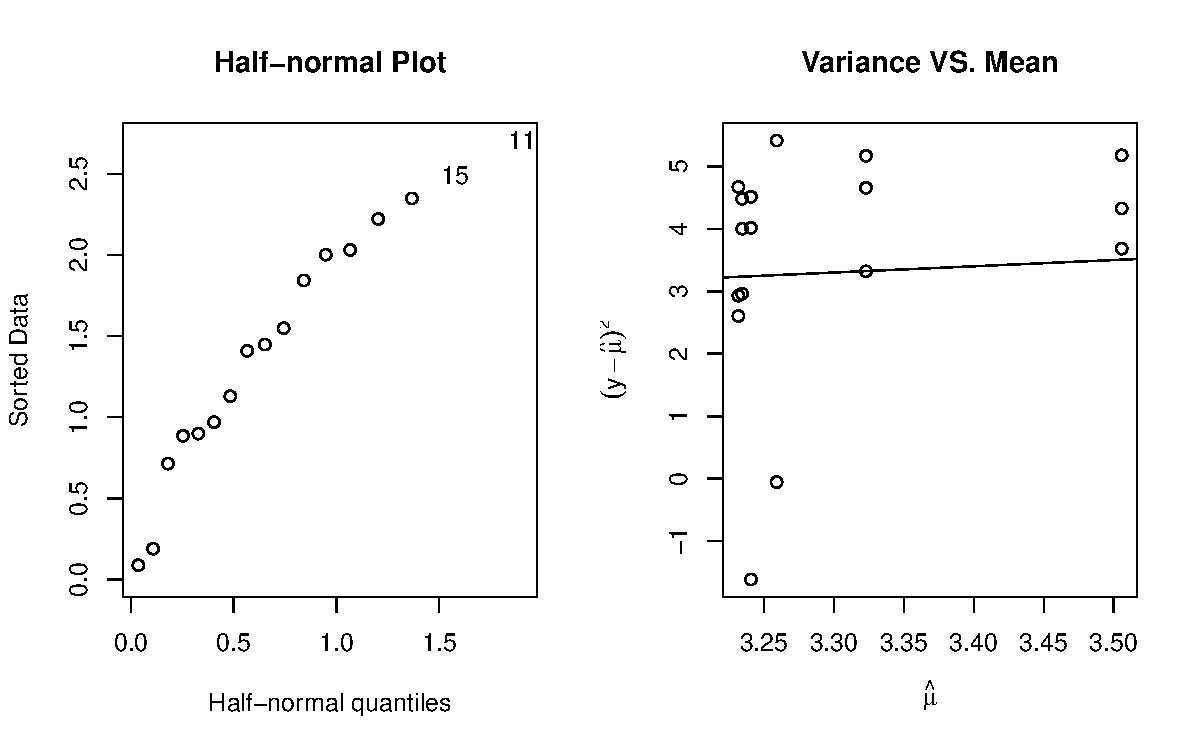
\includegraphics[width=1\linewidth]{figure/p2_2-1} 

}



\end{knitrout}

After removing case 12 from the dataset, the resulting residual deviance is 46.35 with 15 degrees of freedom which still indicates an ill-fitting model if the Poisson is the correct model for the response. Then we check the "Variance vs Mean" plot, we see that the estimated variance is larger than the corresponding mean, suggesting that over-dispersion exists in this model. So that we can correct the model by calculating the dispersion parameter, and then summarize the model under the dispersion parameter.

\begin{knitrout}
\definecolor{shadecolor}{rgb}{1, 1, 1}\color{fgcolor}\begin{kframe}
\begin{alltt}
\hlstd{dp} \hlkwb{<-} \hlkwd{sum}\hlstd{(}\hlkwd{residuals}\hlstd{(m1,} \hlkwc{type} \hlstd{=} \hlstr{"pearson"}\hlstd{)} \hlopt{^} \hlnum{2}\hlstd{)} \hlopt{/} \hlstd{m1}\hlopt{$}\hlstd{df.res}
\hlkwd{summary}\hlstd{(m1,} \hlkwc{dispersion} \hlstd{= dp)}
\end{alltt}
\begin{verbatim}
## 
## Call:
## glm(formula = colonies ~ dose, family = poisson, data = data1)
## 
## Deviance Residuals: 
##      Min        1Q    Median        3Q       Max  
## -2.49190  -1.54866   0.08807   1.40904   2.70520  
## 
## Coefficients:
##              Estimate Std. Error z value Pr(>|z|)    
## (Intercept) 3.2317358  0.1021177  31.647   <2e-16 ***
## dose        0.0002739  0.0002100   1.305    0.192    
## ---
## Signif. codes:  0 '***' 0.001 '**' 0.01 '*' 0.05 '.' 0.1 ' ' 1
## 
## (Dispersion parameter for poisson family taken to be 3.078062)
## 
##     Null deviance: 51.379  on 16  degrees of freedom
## Residual deviance: 46.347  on 15  degrees of freedom
## AIC: 136.95
## 
## Number of Fisher Scoring iterations: 4
\end{verbatim}
\begin{alltt}
\hlkwd{drop1}\hlstd{(m1,} \hlkwc{test} \hlstd{=} \hlstr{"F"}\hlstd{)}
\end{alltt}
\begin{verbatim}
## Single term deletions
## 
## Model:
## colonies ~ dose
##        Df Deviance    AIC F value Pr(>F)
## <none>      46.347 136.95               
## dose    1   51.379 139.98  1.6286 0.2213
\end{verbatim}
\end{kframe}
\end{knitrout}

\problem{7}
The dataset esdcomp was recorded on 44 doctors working in an emergency service at a hospital to study the factors affecting the number of complaints received. Build a model for the number of complaints received and write a report on your conclusions.

\solution
\begin{knitrout}
\definecolor{shadecolor}{rgb}{1, 1, 1}\color{fgcolor}\begin{kframe}
\begin{alltt}
\hlstd{data} \hlkwb{<-} \hlstd{esdcomp}
\hlstd{m1} \hlkwb{<-} \hlkwd{glm}\hlstd{(complaints} \hlopt{~} \hlstd{.,} \hlkwc{family} \hlstd{= poisson,} \hlkwc{data} \hlstd{= data)}
\hlkwd{summary}\hlstd{(m1)}
\end{alltt}
\begin{verbatim}
## 
## Call:
## glm(formula = complaints ~ ., family = poisson, data = data)
## 
## Deviance Residuals: 
##     Min       1Q   Median       3Q      Max  
## -1.8989  -0.9193  -0.3835   0.4981   1.8221  
## 
## Coefficients:
##               Estimate Std. Error z value Pr(>|z|)   
## (Intercept) -0.0803448  1.1542122  -0.070  0.94450   
## visits       0.0009499  0.0003386   2.806  0.00502 **
## residencyY  -0.2319740  0.2029388  -1.143  0.25301   
## genderM      0.1122391  0.2235043   0.502  0.61554   
## revenue     -0.0033827  0.0041553  -0.814  0.41560   
## hours       -0.0001569  0.0006634  -0.237  0.81298   
## ---
## Signif. codes:  0 '***' 0.001 '**' 0.01 '*' 0.05 '.' 0.1 ' ' 1
## 
## (Dispersion parameter for poisson family taken to be 1)
## 
##     Null deviance: 89.447  on 43  degrees of freedom
## Residual deviance: 49.995  on 38  degrees of freedom
## AIC: 184.77
## 
## Number of Fisher Scoring iterations: 5
\end{verbatim}
\begin{alltt}
\hlkwd{drop1}\hlstd{(m1,}\hlkwc{test} \hlstd{=} \hlstr{"F"}\hlstd{)}
\end{alltt}
\begin{verbatim}
## Single term deletions
## 
## Model:
## complaints ~ visits + residency + gender + revenue + hours
##           Df Deviance    AIC F value  Pr(>F)  
## <none>         49.995 184.78                  
## visits     1   57.568 190.35  5.7561 0.02144 *
## residency  1   51.319 184.10  1.0061 0.32219  
## gender     1   50.251 183.03  0.1944 0.66177  
## revenue    1   50.665 183.44  0.5094 0.47974  
## hours      1   50.051 182.83  0.0425 0.83778  
## ---
## Signif. codes:  0 '***' 0.001 '**' 0.01 '*' 0.05 '.' 0.1 ' ' 1
\end{verbatim}
\begin{alltt}
\hlkwd{par}\hlstd{(}\hlkwc{mfrow} \hlstd{=} \hlkwd{c}\hlstd{(}\hlnum{1}\hlstd{,} \hlnum{2}\hlstd{))}
\hlkwd{halfnorm}\hlstd{(}\hlkwd{residuals}\hlstd{(m1),} \hlkwc{main} \hlstd{=} \hlstr{"Half-normal Plot"}\hlstd{)}
\hlkwd{plot}\hlstd{(}\hlkwd{log}\hlstd{(}\hlkwd{fitted}\hlstd{(m1)),} \hlkwd{log}\hlstd{((data}\hlopt{$}\hlstd{complaints} \hlopt{-} \hlkwd{fitted}\hlstd{(m1))}\hlopt{^}\hlnum{2}\hlstd{),}
     \hlkwc{xlab} \hlstd{=} \hlkwd{expression}\hlstd{(}\hlkwd{hat}\hlstd{(mu)),} \hlkwc{ylab} \hlstd{=} \hlkwd{expression}\hlstd{((y} \hlopt{-} \hlkwd{hat}\hlstd{(mu))}\hlopt{^}\hlnum{2}\hlstd{),}
     \hlkwc{main} \hlstd{=} \hlstr{"Variance VS. Mean"}\hlstd{)}
\hlkwd{abline}\hlstd{(}\hlnum{0}\hlstd{,}\hlnum{1}\hlstd{)}
\end{alltt}
\end{kframe}

{\centering 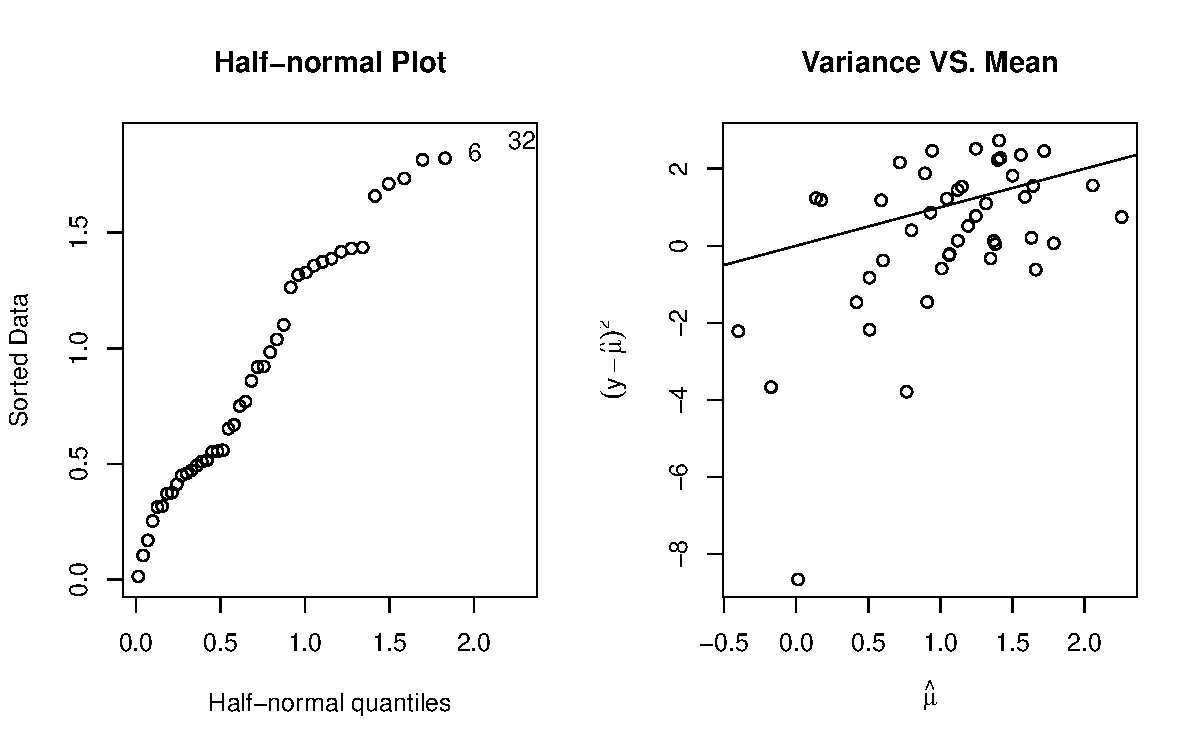
\includegraphics[width=1\linewidth]{figure/p7-1} 

}



\end{knitrout}

First we try to build a Poisson regression model to explain the number of complaints received. The resulting residual deviance is 49.99 on 38 degrees of freedom, suggesting that this is an ill-fitting model. Then we draw Half-normal plot to check outliers. However, the Half-normal plot doesn't suggest strong evidence of the existence of outliers. We conclude that maybe the model itself has some problem, so before adding interactions or polynomial terms, we determine to try negative-binomial model as follows.

\begin{knitrout}
\definecolor{shadecolor}{rgb}{1, 1, 1}\color{fgcolor}\begin{kframe}
\begin{alltt}
\hlstd{m_nb1} \hlkwb{<-} \hlkwd{glm.nb}\hlstd{(complaints} \hlopt{~} \hlstd{.,} \hlkwc{data} \hlstd{= data)}
\hlkwd{summary}\hlstd{(m_nb1)}
\end{alltt}
\begin{verbatim}
## 
## Call:
## glm.nb(formula = complaints ~ ., data = data, init.theta = 27.92769821, 
##     link = log)
## 
## Deviance Residuals: 
##     Min       1Q   Median       3Q      Max  
## -1.8719  -0.8623  -0.3626   0.4896   1.6892  
## 
## Coefficients:
##               Estimate Std. Error z value Pr(>|z|)  
## (Intercept) -0.1363173  1.2307676  -0.111   0.9118  
## visits       0.0009061  0.0003720   2.436   0.0149 *
## residencyY  -0.2165030  0.2174302  -0.996   0.3194  
## genderM      0.1205147  0.2374894   0.507   0.6118  
## revenue     -0.0030832  0.0044565  -0.692   0.4890  
## hours       -0.0001054  0.0007158  -0.147   0.8829  
## ---
## Signif. codes:  0 '***' 0.001 '**' 0.01 '*' 0.05 '.' 0.1 ' ' 1
## 
## (Dispersion parameter for Negative Binomial(27.9277) family taken to be 1)
## 
##     Null deviance: 79.218  on 43  degrees of freedom
## Residual deviance: 44.919  on 38  degrees of freedom
## AIC: 186.54
## 
## Number of Fisher Scoring iterations: 1
## 
## 
##               Theta:  27.9 
##           Std. Err.:  58.8 
## 
##  2 x log-likelihood:  -172.538
\end{verbatim}
\begin{alltt}
\hlkwd{drop1}\hlstd{(m_nb1)}
\end{alltt}
\begin{verbatim}
## Single term deletions
## 
## Model:
## complaints ~ visits + residency + gender + revenue + hours
##           Df Deviance    AIC
## <none>         44.919 184.54
## visits     1   50.912 188.53
## residency  1   45.914 183.53
## gender     1   45.183 182.80
## revenue    1   45.400 183.02
## hours      1   44.941 182.56
\end{verbatim}
\end{kframe}
\end{knitrout}

Here we see for the negative-binomial model, the resulting residual deviance is 44.92 on 38 degrees of freedom, which improves a lot compared with the Poisson regression model. Then, from the anova analysis above we see that there are some coefficients that are not significant enough, so that the full model might be redundant. Hence we can try to remove some insignificant predictors in terms of AIC.

\begin{knitrout}
\definecolor{shadecolor}{rgb}{1, 1, 1}\color{fgcolor}\begin{kframe}
\begin{alltt}
\hlstd{m_nb0} \hlkwb{<-} \hlkwd{glm.nb}\hlstd{(complaints} \hlopt{~} \hlnum{1}\hlstd{,} \hlkwc{data} \hlstd{= data)}
\hlstd{m_AIC} \hlkwb{<-} \hlkwd{step}\hlstd{(m_nb1,} \hlkwc{scope} \hlstd{=} \hlkwd{list}\hlstd{(}\hlkwc{upper} \hlstd{= m_nb1,} \hlkwc{lower} \hlstd{= m_nb0),}
              \hlkwc{trace} \hlstd{=} \hlnum{FALSE}\hlstd{,} \hlkwc{direction} \hlstd{=} \hlstr{"both"}\hlstd{)}
\hlkwd{summary}\hlstd{(m_AIC)}
\end{alltt}
\begin{verbatim}
## 
## Call:
## glm.nb(formula = complaints ~ visits + residency, data = data, 
##     init.theta = 21.56289501, link = log)
## 
## Deviance Residuals: 
##     Min       1Q   Median       3Q      Max  
## -1.8965  -0.8423  -0.3588   0.6096   1.8203  
## 
## Coefficients:
##               Estimate Std. Error z value Pr(>|z|)    
## (Intercept) -0.6828905  0.4292719  -1.591    0.112    
## visits       0.0007897  0.0001563   5.053 4.34e-07 ***
## residencyY  -0.2931900  0.1869824  -1.568    0.117    
## ---
## Signif. codes:  0 '***' 0.001 '**' 0.01 '*' 0.05 '.' 0.1 ' ' 1
## 
## (Dispersion parameter for Negative Binomial(21.5629) family taken to be 1)
## 
##     Null deviance: 76.692  on 43  degrees of freedom
## Residual deviance: 44.327  on 41  degrees of freedom
## AIC: 181.24
## 
## Number of Fisher Scoring iterations: 1
## 
## 
##               Theta:  21.6 
##           Std. Err.:  35.7 
## 
##  2 x log-likelihood:  -173.239
\end{verbatim}
\begin{alltt}
\hlkwd{drop1}\hlstd{(m_AIC)}
\end{alltt}
\begin{verbatim}
## Single term deletions
## 
## Model:
## complaints ~ visits + residency
##           Df Deviance    AIC
## <none>         44.327 179.24
## visits     1   71.357 204.27
## residency  1   46.820 179.73
\end{verbatim}
\end{kframe}
\end{knitrout}

Here we see the reduced model in terms of AIC has residual deviance 44.33 on 41 degrees of freedom, which further improves the previous model in terms of the interpretability. 

The positive coefficient of \m{visits} suggests that the more a patient visits doctors, the more complaints will be made by the patient. Note that the coefficient for \m{residencyY} is negative, which indicates that doctors who have experience in the residency training are more likely to have less complaints from the patients.


\end{document}
